\documentclass[a5paper, 10pt]{article}

% Текст
\usepackage[utf8]{inputenc} % UTF-8 кодировка
\usepackage[russian]{babel} % Русский язык
\usepackage{indentfirst} % красная строка в первом параграфе в главе
% Отображение страниц
\usepackage{geometry} % размеры листа и отступов
\usepackage{listings}
\usepackage{color}

\geometry{
	left=12mm,
	top=25mm,
	right=15mm,
	bottom=17mm,
	marginparsep=0mm,
	marginparwidth=0mm,
	headheight=10mm,
	headsep=7mm,
	nofoot}
\usepackage{afterpage,fancyhdr} % настройка колонтитулов
\pagestyle{fancy}
\fancypagestyle{style}{ % создание нового стиля style
	\fancyhf{} % очистка колонтитулов
	\fancyhead[LO, RE]{Типовой расчет № 1} % название документа наверху
	\fancyhead[RO, LE]{Функции нескольких переменных} % название section наверху
	\fancyfoot[RO, LE]{\thepage} % номер страницы справа внизу на нечетных и слева внизу на четных
	\renewcommand{\headrulewidth}{0.25pt} % толщина линии сверху
	\renewcommand{\footrulewidth}{0pt} % толцина линии снизу
}
\fancypagestyle{plain}{ % создание нового стиля plain -- полностью пустого
	\fancyhf{}
	\renewcommand{\headrulewidth}{0pt}
}
\fancypagestyle{title}{ % создание нового стиля title -- для титульной страницы
	\fancyhf{}
	\fancyhead[C]{{\footnotesize
			Министерство образования и науки Российской Федерации\\
			Федеральное государственное автономное образовательное учреждение высшего образования
	}}
	\fancyfoot[C]{{\large 
			Санкт-Петербург, 2023-2024
	}}
	\renewcommand{\headrulewidth}{0pt}
}

% Математика
\usepackage{amsmath, amsfonts, amssymb, amsthm} % Набор пакетов для математических текстов
%\usepackage{dmvnbase} % мехматовский пакет latex-сокращений
\usepackage{cancel} % зачеркивание для сокращений
% Рисунки и фигуры
\usepackage[pdftex]{graphicx} % вставка рисунков
\usepackage{wrapfig, subcaption} % вставка фигур, обтекая текст
\usepackage{caption} % для настройки подписей
\captionsetup{figurewithin=none,labelsep=period, font={small,it}} % настройка подписей к рисункам
% Рисование
\usepackage{tikz} % рисование
\usepackage{circuitikz}
\usepackage{pgfplots} % графики
% Таблицы
\usepackage{multirow} % объединение строк
\usepackage{multicol} % объединение столбцов
% Остальное
\usepackage[unicode, pdftex]{hyperref} % гиперссылки
\usepackage{enumitem} % нормальное оформление списков
\setlist{itemsep=0.15cm,topsep=0.15cm,parsep=1pt} % настройки списков
% Теоремы, леммы, определения...
\theoremstyle{definition}
\newtheorem{Def}{Определение}
\newtheorem*{Axiom}{Аксиома}
\theoremstyle{plain}
\newtheorem{Th}{Теорема}
\newtheorem{Lem}{Лемма}
\newtheorem{Cor}{Следствие}
\newtheorem{Ex}{Пример}
\theoremstyle{remark}
\newtheorem*{Note}{Замечание}
\newtheorem*{Solution}{Решение}
\newtheorem*{Proof}{Доказательство}
% Свои команды
\newcommand{\comb}[1]{\left[\hspace{-4pt}\begin{array}{l}#1\end{array}\right.\hspace{-5pt} } % совокупность уравнений
% Титульный лист
\usepackage{csvsimple-l3}
\newcommand*{\titlePage}{
	\thispagestyle{title}
	\begingroup
	\begin{center}
		%		{\footnotesize
			%			Министерство образования и науки Российской Федерации\\
			%			Федеральное государственное автономное образовательное учреждение высшего образования
			%		}
		%		
		\vspace*{6ex}
		
		{\small
			САНКТ-ПЕТЕРБУРГСКИЙ НАЦИОНАЛЬНЫЙ ИССЛЕДОВАТЕЛЬСКИЙ УНИВЕРСИТЕТ ИТМО	
		}
		
		\vspace*{2ex}
		
		{\normalsize
			Факультет систем управления и робототехники
		}
		
		\vspace*{15ex}
		
		{\Large \bfseries 
			Типовой расчет и лабораторная работа № 1
		}
\vspace*{2ex}
	{\Large \bfseries 
			
"Функции нескольких переменных "
		}
\vspace*{2ex}
		
		{\normalsize
			по дисциплине Математический анализ
		}

	\end{center}
	\vspace*{20ex}
	\begin{flushright}
		{\large 
			\underline{Выполнила}: студентка гр. \textbf{R3238}\\
			\begin{flushright}
				\textbf{Нечаева А. А.}\\
			\end{flushright}
		}
		
		\vspace*{5ex}
		
		{\large 
			\underline{Преподаватель}: \textit{Бойцев Антон Александрович}
		}
	\end{flushright}	
	\newpage
	\setcounter{page}{1}
	\endgroup}

\begin{document}
	\titlePage
	\pagestyle{style}
\newpage

\section{задание.}
\textit{Найти частные производные данной функции $f(x, y)$ в точке $(0, 0)$. Выяснить, является ли функция дифференцируемой в точке $(0, 0)$. Найти её дифференциал. \textbf{Пункт 2}.}
\begin{equation}
f(x, y) = y + \cos \sqrt[3]{x^2 + y^2}
\end{equation}
\subsection{Частные производные}

\begin{equation}
\frac{\partial f}{\partial x} (x_0, y_0) = \lim_{\Delta x \to 0} \frac{\Delta_x f}{\Delta x} = \lim_{\Delta x \to 0} \frac{f ( x_0 + \Delta x, y_0) - f(x_0, y_0)}{\Delta x}
\end{equation}
\\

Производная по $x$ в точке $(0, 0)$:
\begin{multline}
\frac{\partial f}{\partial x} (0, 0) = \lim_{\Delta x \to 0} \frac{\cos \sqrt[3]{( \Delta x)^2} - \cos 0}{\Delta x} = 
-2 \lim_{\Delta x \to 0} \frac{\sin^2  \frac{ \sqrt[3]{( \Delta x)^2}}{2}}{\Delta x} =\\
= -2 \lim_{\Delta x \to 0} \frac{\sin^2  \frac{ \sqrt[3]{( \Delta x)^2}}{2} \sqrt[3]{ \Delta x}}{4 \left(\frac{ \sqrt[3]{( \Delta x)^2}}{2} \right)^2} = 0
\end{multline}


Производная по $y$ в точке $(0, 0)$:
\begin{multline}
\frac{\partial f}{\partial y} (0, 0) = \lim_{\Delta y \to 0} \frac{\Delta y + \cos \sqrt[3]{( \Delta y)^2} - \cos 0}{\Delta y} = 
\lim_{\Delta y \to 0} \left(1 +  \frac{\cos \sqrt[3]{( \Delta y)^2} - 1}{\Delta y} \right) =\\
= 1 - 2 \lim_{\Delta y \to 0} \frac{\sin^2  \frac{ \sqrt[3]{( \Delta y)^2}}{2}}{\Delta y} 
=1 -2 \lim_{\Delta y \to 0} \frac{\sin^2  \frac{ \sqrt[3]{( \Delta y)^2}}{2} \sqrt[3]{ \Delta y}}{4 \left(\frac{ \sqrt[3]{( \Delta y)^2}}{2} \right)^2} = 1
\end{multline}


\subsection{Дифференцируемость в точке  $(0, 0)$}
Функция будет дифференцируема в точке $\left(0;0 \right)$, если для ее приращения в этой точке выполняется равенство:
\begin{equation}
\Delta f (0;0) = \frac{\partial f}{\partial x} (0;0) \cdot \Delta x +  \frac{\partial f}{\partial y} (0;0) \cdot \Delta y + o(\rho)\, ,
\end{equation}
где $\rho = \sqrt{\Delta x^2 + \Delta y^2}$.\\
Запишем формулу, подставив в нее выше найденные производные:
\begin{equation}
\Delta f (0;0) = 0 \cdot \Delta x +  1 \cdot \Delta y + o( \sqrt{\Delta x^2 + \Delta y^2}) = \Delta y + o( \sqrt{\Delta x^2 + \Delta y^2})
\end{equation}
\textit{\textbf{Ответ:}} функция дифференцируема в точке $(0, 0)$.

\subsection{Дифференциал}

\begin{equation}
df = \frac{\partial f}{\partial x} dx + \frac{\partial f}{\partial y} dy
\end{equation}
Найдем частные производные:

\begin{equation}
\frac{\partial f}{\partial x} = \left( y + \cos \sqrt[3]{x^2 + y^2} \right)'_x = -\frac{2x}{3} \frac{\sin \sqrt[3]{x^2 + y^2}}{\sqrt[3]{ \left( x^2 + y^2 \right)^2}}
\end{equation}

\begin{equation}
\frac{\partial f}{\partial y} = \left( y + \cos \sqrt[3]{x^2 + y^2} \right)'_y = 1 -\frac{2y}{3} \frac{\sin \sqrt[3]{x^2 + y^2}}{\sqrt[3]{ \left( x^2 + y^2 \right)^2}}
\end{equation}
Терерь запишем полный дифференциал:

\begin{equation}
df =  -\frac{2x}{3} \frac{\sin \sqrt[3]{x^2 + y^2}}{\sqrt[3]{ \left( x^2 + y^2 \right)^2}} dx + \left( 1 -\frac{2y}{3} \frac{\sin \sqrt[3]{x^2 + y^2}}{\sqrt[3]{ \left( x^2 + y^2 \right)^2}}  \right) dy
\end{equation}

\newpage

\section{задание}
\textit{Найти производную данной функции в направлении данного вектора в заданной точке $M$. \textbf{Пункт 8}.}

\begin{equation}
f(x, y, z) = \exp(x + 2xy + 3xyz)
\end{equation}
по направлению внутренней нормали к поверхности $x^2 + y^2 + z^2 + 2z = 1$, $M \left( \frac{1}{2}, \frac{\sqrt{3}}{2}, 0 \right)$\\
\\
Найдем уравнение касательной плоскости к поверхности $x^2 + y^2 + z^2 + 2z = 1$ в точке $M \left( \frac{1}{2}, \frac{\sqrt{3}}{2}, 0 \right)$:

\begin{equation}
F'_x \left( M \right) \cdot (x - x_0) + F'_y \left( M \right) \cdot (y - y_0) + F'_z \left( M \right) \cdot (z - z_0) = 0
\end{equation}

\begin{equation}
F'_x = \left(  x^2 + y^2 + z^2 + 2z - 1 \right)'_x = 2x
\end{equation}

\begin{equation}
F'_y = \left(  x^2 + y^2 + z^2 + 2z - 1 \right)'_y = 2y
\end{equation}

\begin{equation}
F'_z = \left(  x^2 + y^2 + z^2 + 2z - 1 \right)'_z = 2z + 2
\end{equation}

\begin{equation}
F'_x  \left( M \right) = 2 \frac{1}{2} = 1
\end{equation}

\begin{equation}
F'_y  \left( M \right) = 2 \frac{\sqrt{3}}{2} = \sqrt{3}
\end{equation}

\begin{equation}
F'_z  \left( M \right) = 2
\end{equation}

Искомая плоскость:
\begin{equation}
x - \frac{1}{2}  +  \sqrt{3} \cdot (y - \frac{\sqrt{3}}{2}) + 2z= 0
\end{equation}

\begin{equation}
x  + \sqrt{3}y + 2z - 2= 0
\end{equation}
\\
Вектор нормали к плоскости $x  + \sqrt{3}y + 2z - 2= 0$ будет выглядеть $\vec{n} = \left( 1, \sqrt{3}, 2 \right)$. Поверхность  $x^2 + y^2 + z^2 + 2z = 1$ представляет собой сферу  $x^2 + y^2 + \left( z + 1\right)^2 = 2$ с центром $O = (0, 0, -1)$ и радиусом $R = \sqrt{2}$. Так как точкой начала вектора $\vec{n}$ является  $M \left( \frac{1}{2}, \frac{\sqrt{3}}{2}, 0 \right)$, а его координаты  $\vec{n} = \left( 1, \sqrt{3}, 2 \right)$, то точкой конца вектора будет $\left(  \frac{3}{2}, \frac{3 \sqrt{3}}{2}, 2 \right)$. То есть вектор $\vec{n} = \left( 1, \sqrt{3}, 2 \right)$ направлен наружу относительно поверхности.\\
\\
Внутренняя нормаль $\vec{n}_{in} = \left( -1, -\sqrt{3}, -2 \right)$. \\
Получим нормированный вектор, по направлению которого будем вычислять производную:
\begin{equation}
\left|\vec{n}_{in}  \right| = \sqrt{1 + 3 + 4} =  \sqrt{8} = 2\sqrt{2}
\end{equation}

\begin{equation}
l = \left( -\frac{1}{2\sqrt{2}}, - \frac{\sqrt{3}}{2\sqrt{2}}, - \frac{1}{\sqrt{2}} \right)
\end{equation}

Вычислим частные производные от $f(x, y, z) = \exp(x + 2xy + 3xyz)$ в точке $M \left( \frac{1}{2}, \frac{\sqrt{3}}{2}, 0 \right)$:

\begin{equation}
f'_x = \left(1 + 2y + 3yz \right) \exp(x + 2xy + 3xyz)
\end{equation}

\begin{equation}
f'_y  = \left( 2x + 3xz \right) \exp(x + 2xy + 3xyz)
\end{equation}

\begin{equation}
f'_z   = 3xy \exp(x + 2xy + 3xyz)
\end{equation}

\begin{equation}
f'_x  \left( M \right) =  \left(1 + 2 \frac{\sqrt{3}}{2} \right) \exp \left( \frac{1}{2} + 2 \frac{1}{2}\frac{\sqrt{3}}{2} \right) =
\left(1 + \sqrt{3} \right) \exp \left( \frac{\sqrt{3} + 1}{2} \right) 
\end{equation}

\begin{equation}
f'_y  \left( M \right) =  \left( 2\frac{1}{2}  \right) \exp \left(\frac{1}{2} + 2\frac{1}{2}\frac{\sqrt{3}}{2} \right) =
\exp \left(\frac{\sqrt{3} + 1}{2} \right)
\end{equation}

\begin{equation}
f'_z  \left( M \right) = 3\frac{1}{2}\frac{\sqrt{3}}{2} \exp \left(\frac{1}{2} + 2\frac{1}{2}\frac{\sqrt{3}}{2} \right) =
\frac{3 \sqrt{3}}{4} \exp \left(\frac{\sqrt{3} + 1}{2} \right)
\end{equation}
\\
Вычислим производную по направлению $l$ в точке $M$:

\begin{multline}
\frac{\partial f}{\partial l} = \left(\left(1 + \sqrt{3} \right) e^{ \frac{\sqrt{3} + 1}{2}} , e^{ \frac{\sqrt{3} + 1}{2}}, \frac{3 \sqrt{3}}{4} e^{ \frac{\sqrt{3} + 1}{2}  } \right)
\begin{pmatrix}
 -\frac{1}{2\sqrt{2}}\\
\\
- \frac{\sqrt{3}}{2\sqrt{2}}\\
\\
- \frac{1}{\sqrt{2}}
\end{pmatrix}
= \\
=   -\frac{1 + \sqrt{3}}{2\sqrt{2}} e^{ \frac{\sqrt{3} + 1}{2}} - \frac{\sqrt{3}}{2\sqrt{2}}  e^{ \frac{\sqrt{3} + 1}{2}}
 - \frac{1.5 \sqrt{3}}{2\sqrt{2}}  e^{ \frac{\sqrt{3} + 1}{2}}  =  - \frac{1 + 3.5 \sqrt{3}}{2\sqrt{2}}  e^{ \frac{\sqrt{3} + 1}{2}} 
\end{multline}

\textit{\textbf{Ответ:}} $ - \frac{1 + 3.5 \sqrt{3}}{2\sqrt{2}}  e^{ \frac{\sqrt{3} + 1}{2}} $





\newpage

\section{задание}
\textit{Произвести указанную замену в данном дифференциальном уравнении. Решить полученное дифференциальное уравнение в новых переменных. Показать, что найденное решение (в исходных переменных) удовлетворяет исходному уравнению. \textbf{Пункт 3}.}\\
\\
$u$ и $v$ -- новые независимые переменные, $w$ -- новая функция. $u=x+y, \, v = x - y, \, w+z = xy,$

\begin{equation}
\frac{\partial^2 z}{\partial x^2} + 2 \frac{\partial^2 z}{\partial x \partial y} + \frac{\partial^2 z}{\partial y^2} = 0
\end{equation}
 $z=z(x, y)$, $w=w(u, v)$, $u = u(x, y)$, $v = v(x, y)$

Для начала найдем все производные второго порядка функции $w$ по переменным $x$ и $y$:
\begin{equation}
w'_x = w'_u \cdot u'_x + w'_v \cdot v'_x = w'_u + w'_v
\end{equation}

% for x
\begin{equation}
w''_{ux}  = w''_{uu} \cdot u'_x + w''_{uv} \cdot v'_x = w''_{uu} + w''_{uv}
\end{equation}

\begin{equation}
w''_{vx}  = w''_{vu} \cdot u'_x + w''_{vv} \cdot v'_x = w''_{vu} + w''_{vv}
\end{equation}

Вторая производная по  $x$:
\begin{equation}
w''_{xx} = w''_{uu} + 2w''_{uv} + w''_{vv}
\end{equation}


\begin{equation}
w'_y = w'_u \cdot u'_y + w'_v \cdot v'_y = w'_u - w'_v
\end{equation}

\begin{equation}
w''_{uy}  = w''_{uu} \cdot u'_y + w''_{uv} \cdot v'_y = w''_{uu} - w''_{uv}
\end{equation}

\begin{equation}
w''_{vy}  = w''_{vu} \cdot u'_y + w''_{vv} \cdot v'_y = w''_{vu} - w''_{vv}
\end{equation}

 Вторая производная по $y$:
\begin{equation}
w''_{yy} = w''_{uu} - 2w''_{uv} + w''_{vv}
\end{equation}

Вторая производная по  $x$ и $y$:

\begin{equation}
w''_{yx} = w''_{xy} =  w''_{uu} -  w''_{vv}
\end{equation}
\\
Теперь выразим $z''_{xx}$,  $z''_{xy}$ и $z''_{yy}$ из $w + z = xy$:
\begin{equation}
z = xy - w
\end{equation}

\begin{equation}
z'_x = y - w'_x
\end{equation}

\begin{equation}
z'_y = x - w'_y
\end{equation}

\begin{equation}
z''_{xx} = - w''_{xx} = - ( w''_{uu} + 2w''_{uv} + w''_{vv})
\end{equation}


\begin{equation}
z''_{xy} = 1 - w''_{xy} = 1 - ( w''_{uu} -  w''_{vv})
\end{equation}

\begin{equation}
z''_{yy} = - w''_{yy} = -( w''_{uu} - 2w''_{uv} + w''_{vv})
\end{equation}
\\
Перепишем исходное уравнение в новых переменных и функции:

\begin{equation}
- ( w''_{uu} + 2w''_{uv} + w''_{vv}) + 2 (1 - ( w''_{uu} -  w''_{vv})) -( w''_{uu} - 2w''_{uv} + w''_{vv}) = 0
\end{equation}
\begin{equation}
- w''_{uu} - 2w''_{uv} - w''_{vv} + 2 -2  w''_{uu} +2  w''_{vv} - w''_{uu} + 2w''_{uv} - w''_{vv} = 0
\end{equation}
\begin{equation}
- w''_{uu}  + 2 -2  w''_{uu}  - w''_{uu}   = 0
\end{equation}
\begin{equation}
4 w''_{uu}  = 2
\end{equation}
\begin{equation}
 w''_{uu}  = \frac{1}{2}
\end{equation}
Решим полученное дифференциальное уравнение:

\begin{equation}
 \frac{d(w')}{du}  = \frac{1}{2}
\end{equation}

\begin{equation}
 d(w')  = \frac{1}{2} du
\end{equation}

\begin{equation}
 \int d(w')  = \int \frac{1}{2} du
\end{equation}

\begin{equation}
 w' =  \frac{u}{2} + C
\end{equation}

\begin{equation}
 dw = \left( \frac{u}{2} + C \right) du
\end{equation}

\begin{equation}
 \int dw =\int  \left( \frac{u}{2} + C \right) du
\end{equation}

\begin{equation}
 w =  \frac{u^2}{4} + Cu + A, \, A = const, \, C = const
\end{equation}

Решение в новых переменных:
\begin{equation}
 w =  \frac{u^2}{4} + Cu + A
\end{equation}

Выполним проверку: вернемся к старым переменным и подставим полученные выражения в исходное равенство:


\begin{equation}
u = x + y
\end{equation}

\begin{equation}
z = xy - w = xy -  \frac{u^2}{4} - Cu - A =  xy -  \frac{( x + y)^2}{4} - C( x + y) - A
\end{equation}

\begin{equation}
\frac{\partial^2 z}{\partial x^2} + 2 \frac{\partial^2 z}{\partial x \partial y} + \frac{\partial^2 z}{\partial y^2} = 0
\end{equation}

\begin{equation}
z'_x = \left(  xy -  \frac{( x + y)^2}{4} - C( x + y) - A \right)'_x = y - \frac{ x + y}{2}  -C = \frac{y}{2} - \frac{ x}{2} -C
\end{equation}

\begin{equation}
z'_y = \left(  xy -  \frac{( x + y)^2}{4} - C( x + y) - A \right)'_y = x - \frac{ x + y}{2}  -C = \frac{x}{2} - \frac{y}{2} -C
\end{equation}

\begin{equation}
z''_{xx} = \left(  \frac{y}{2} - \frac{ x}{2} -C \right)'_x =  - \frac{ 1}{2}
\end{equation}

\begin{equation}
z''_{xy} = \left(  \frac{y}{2} - \frac{ x}{2} -C \right)'_y =   \frac{ 1}{2}
\end{equation}

\begin{equation}
z''_{yy} = \left(  \frac{x}{2} - \frac{y}{2} - \right)'_y =  - \frac{ 1}{2}
\end{equation}

Подставим полученные выражения в исходное уравнение уравнение:

\begin{equation}
- \frac{ 1}{2} + 2\frac{ 1}{2} - \frac{ 1}{2} = 0
\end{equation}
Получили верное равенство.\\

\textit{\textbf{Ответ:}} $ w =  \frac{u^2}{4} + Cu + A $


\newpage

\section{задание}
\textit{Доказать, что уравнение $F(x,y)=0, \, F=(F_1, F_2)$ задает неявно дифференцируемое отображение $y=f(x), \, y=(y_1, y_2), \, x = (x_1, \, x_2)$ в окрестности точки $M(x_1, x_2, y_1, y_2)$. Найти производную этого отображения в точке $M$ (матрица Якоби) и одну (любую на выбор) из производных второго порядка $\frac{\partial f_i}{\partial x_j}$ в точке $M$. \textbf{Пункт 3}.}

\begin{equation}
\begin{cases}
F_1 (x, y) = x_1 + x_2 + y_1 + 2y_2 -5,\\
F_2 (x, y) = x^3_1 + x^2_2 +y^4_1+y^4_2-4,
\end{cases}
M(1, 1, 1, 1)
\end{equation}



\begin{equation}
\begin{cases}
F_1(M) = 1 + 1 + 1 + 2 - 5 = 0\\
F_2(M) = 1 + 1 + 1 + 1 -4 = 0
\end{cases}
\end{equation}

\begin{equation}
\begin{cases}
y_1 = f_1 (x) = f_1 (x_1, x_2)\\
y_2 = f_2 (x) = f_2 (x_1, x_2)
\end{cases}
\end{equation}
\begin{equation}
|F'_y| = 
\begin{vmatrix} 
\frac{\partial F_1}{\partial y_1} & \frac{\partial F_1}{\partial y_2}\\
\\
\frac{\partial F_2}{\partial y_1} & \frac{\partial F_2}{\partial y_2}
\end{vmatrix}
=
\begin{vmatrix} 
1 & 2 \\
4y_1^3 & 4y_2^3
\end{vmatrix}
=
\begin{vmatrix} 
1 & 2 \\
4 & 4
\end{vmatrix}
=-4 \neq 0
\end{equation}
Следовательно,  уравнение $F(x,y)=0, \, F=(F_1, F_2)$ задает неявно дифференцируемое отображение $y=f(x), \, y=(y_1, y_2), \, x = (x_1, \, x_2)$ в окрестности точки $M(x_1, x_2, y_1, y_2)$.

\begin{equation}
f'_x (M) = - \frac{F'_x (M)}{F'_y (M)}
\end{equation}

\begin{equation}
F'_x (M)= 
\begin{pmatrix} 
\frac{\partial F_1}{\partial x_1} & \frac{\partial F_1}{\partial x_2}\\
\\
\frac{\partial F_2}{\partial x_1} & \frac{\partial F_2}{\partial x_2}
\end{pmatrix}
=
\begin{pmatrix} 
1 & 1 \\
3x_1^2 & 2x_2
\end{pmatrix}
=
\begin{pmatrix} 
1 & 1 \\
3 & 2
\end{pmatrix}
\end{equation}


\begin{equation}
(F'_y)^{-1} (M) = 
\begin{pmatrix} 
1 & 2 \\
4 & 4
\end{pmatrix}^{-1}
=
\begin{pmatrix} 
-1 & \frac{1}{2} \\
\\
1 & - \frac{1}{4}
\end{pmatrix}
\end{equation}

\begin{equation}
f'_x (M) = - F'_x (F'_y)^{-1}  =
\begin{pmatrix} 
1 & 1 \\
3 & 2
\end{pmatrix}
\begin{pmatrix} 
-1 & \frac{1}{2} \\
\\
1 & - \frac{1}{4}
\end{pmatrix}
= -
\begin{pmatrix}
0 & \frac{1}{4}\\
-1 & 1
\end{pmatrix}
=
\begin{pmatrix}
0 & -\frac{1}{4}\\
1 & -1
\end{pmatrix}
\end{equation}

Найдем производную второго порядка $\frac{\partial ^ 2 f_1}{\partial x_1^2}$
\begin{equation}
F'_x =
\begin{pmatrix} 
1 & 1 \\
3x_1^2 & 2x_2
\end{pmatrix}
\end{equation}

\begin{equation}
(F'_y)^{-1} =
\begin{pmatrix} 
1 & 2 \\
4y_1^3 & 4y_2^3
\end{pmatrix}^{-1}
=
\frac{1}{4y_2^3 - 8y_1^3}
\begin{pmatrix} 
4 y_2^3 & -2 \\
-4y_1^3 & 1
\end{pmatrix}
\end{equation}

\begin{equation}
f'_x =
-\frac{1}{4y_2^3 - 8y_1^3}
\begin{pmatrix} 
1 & 1 \\
3x_1^2 & 2x_2
\end{pmatrix}
\begin{pmatrix} 
4 y_2^3 & -2 \\
-4y_1^3 & 1
\end{pmatrix}
\end{equation}

Значению $\frac{\partial f_1}{\partial x_1}$ соответствует выражение, стоящее на позиции $[0, 0]$ в полученной матрице $f'_x$:
\begin{equation}
\frac{\partial f_1}{\partial x_1} = \frac{ y^3_1 - y^3_2 }{y_2^3 - 2y_1^3}
\end{equation}

\begin{equation}
\frac{\partial ^ 2 f_1}{\partial x_1^2} = 0
\end{equation}










\newpage

\section{задание}
\textit{С помощью метода Лагранжа исследовать функцию на условный экстремум при данном уравнении связи. \textbf{Пункт 2}.}

\begin{equation}
f(x, y, z) = x^2+2y^2+3z^2, \, x + 2y+3z=0, \, x^2 +y^2+z^2=1
\end{equation}
Запишем вид функции Лагранжа:
\begin{equation}
L = u(x, y, z) - \lambda_1 \phi_1 (x, y, z) - \lambda_2 \phi_2 (x, y, z)
\end{equation}

\begin{equation}
L = x^2+2y^2+3z^2  - \lambda_1 \left(  x + 2y+3z \right) - \lambda_2 \left( x^2 +y^2+z^2 - 1   \right)
\end{equation}

\begin{equation}
\begin{cases}
L'_x = 2x - \lambda_1 -2 \lambda_2 x = 0\\
L'_y = 4y  - 2\lambda_1  - 2\lambda_2 y = 0\\
L'_z = 6z  - 3 \lambda_1  - 2\lambda_2 z = 0\\
L'_{\lambda_1}=   x + 2y+3z = 0\\
L'_ { \lambda_2} =  x^2 +y^2+z^2 - 1 = 0
\end{cases}
\end{equation}

\begin{equation}
L'_z - L'_y - L'_x = 6z-4y-2x -2 \lambda_2 (z - y - x) = 0
\end{equation}
\begin{equation}
6z-4y-2x -2 \lambda_2 (z - y - x) = 0 \Leftrightarrow 3z-2y-x = \lambda_2 (z - y - x)
\end{equation}

\begin{equation}
\lambda_2  = \frac{ 3z-2y-x}{z - y - x}
\end{equation}
Воспользовавшись численным методом решения получаем следующие решения системы уравнений:
\begin{equation}
1) \, \, \, 
\begin{pmatrix}
x \\
y \\
z \\
\lambda_1\\
\lambda_2\\
\end{pmatrix}
=
\begin{pmatrix}
0.959 \\
-0.233 \\
-0.164 \\
-0.207\\
1.108\\
\end{pmatrix}
\end{equation}

\begin{equation}
2) \, \, \, 
\begin{pmatrix}
x \\
y \\
z \\
\lambda_1\\
\lambda_2\\
\end{pmatrix}
=
\begin{pmatrix}
-0.959 \\
0.233 \\
0.164 \\
0.207\\
1.108\\
\end{pmatrix}
\end{equation}

\begin{equation}
3) \, \, \, 
\begin{pmatrix}
x \\
y \\
z \\
\lambda_1\\
\lambda_2\\
\end{pmatrix}
=
\begin{pmatrix}
0.099 \\
0.813 \\
-0.575 \\
-0.260\\
2.320\\
\end{pmatrix}
\end{equation}

\begin{equation}
4) \, \, \, 
\begin{pmatrix}
x \\
y \\
z \\
\lambda_1\\
\lambda_2\\
\end{pmatrix}
=
\begin{pmatrix}
-0.099 \\
-0.813 \\
0.575 \\
0.260\\
2.320\\
\end{pmatrix}
\end{equation}
\\

\textit{\textbf{Рассмотрим случай 1) :}}
\begin{multline}
L(x, y, z) = x^2+2y^2+3z^2  + 0.207  \left(  x + 2y+3z \right) - 1.108 \left( x^2 +y^2+z^2 - 1   \right) = \\
= -0.108 x^2 + 0.892 y^2 + 1.892 z^2 + 0.207  \left(  x + 2y+3z \right)  + 1.108
\end{multline}

\begin{equation}
d^2L = 
\begin{pmatrix}
-0.216 & 0 & 0\\
0 & 1.784 & 0\\
0 & 0 & 3.784
\end{pmatrix}
\Rightarrow d^2L = -0.216 d x^ 2 + 1.784 dy^2 + 3.784 dz^2
\end{equation}

Из уравнений связи выразим $dx$ и $dy$:
\begin{multline}
\begin{cases}
 x + 2y+3z=0, \\
 x^2 +y^2+z^2=1
\end{cases}
\Rightarrow
\begin{cases}
 dx + 2dy+3dz=0, \\
 2xdx +2ydy+2zdz=0
\end{cases}
\Rightarrow \\
\begin{cases}
 dx = - 2dy-3dz, \\
 dy= \frac{3x - z}{y - 2x}dz
\end{cases}
\Rightarrow 
\begin{cases}
 dx = - 2 \frac{3x - z}{y - 2x}dz-3dz, \\
 dy= \frac{3x - z}{y - 2x}dz
\end{cases}
\Rightarrow 
\begin{cases}
 dx = \frac{3y- 2z}{2x -y}dz, \\
 dy= \frac{3x - z}{y - 2x}dz
\end{cases}
\end{multline}

\begin{multline}
 d^2L = -0.216 \left( \frac{-3\cdot 0.233 +2 \cdot 0.164}{2\cdot 0.959 +0.233} \right)^ 2dz^ 2  + 1.784  \left( \frac{3\cdot 0.959 + 0.164}{-0.233 - 2\cdot 0.959}\right)^ 2dz^ 2  + \\
+ 3.784 dz^2 = 3.780 dz^2 + 1.784  \left( \frac{3\cdot 0.959 + 0.164}{-0.233 - 2\cdot 0.959}\right)^ 2dz^ 2 > 0
\end{multline}
Следовательно, $(0.959, -0.233, -0.164 )$ -- \textit{\textbf{точка условного минимума}}.



\newpage
\textit{\textbf{Рассмотрим случай 2) :}}
\begin{multline}
 d^2L = -0.216 \left( \frac{3\cdot 0.233 -2 \cdot 0.164}{-2\cdot 0.959 -0.233} \right)^ 2dz^ 2  + 1.784  \left( \frac{-3\cdot 0.959 - 0.164}{0.233 + 2\cdot 0.959}\right)^ 2dz^ 2  + \\
+ 3.784 dz^2 = 3.780 dz^2 + 1.784  \left( \frac{-3\cdot 0.959 - 0.164}{0.233 + 2\cdot 0.959}\right)^ 2dz^ 2 > 0
\end{multline}
Следовательно, $(-0.959, 0.233, 0.164 )$ -- \textit{\textbf{точка условного минимума}}.
\\
\\
\textit{\textbf{Рассмотрим случай 3) :}}




\begin{multline}
L(x, y, z) = x^2+2y^2+3z^2  + 0.260  \left(  x + 2y+3z \right) - 2.320 \left( x^2 +y^2+z^2 - 1   \right) = \\
= -1.320 x^2 - 0.320 y^2 +  0.680 z^2 + 0.260  \left(  x + 2y+3z \right)  + 2.320
\end{multline}

\begin{equation}
d^2L = 
\begin{pmatrix}
-2.640 & 0 & 0\\
0 & -0.640 & 0\\
0 & 0 & 1.360
\end{pmatrix}
\Rightarrow d^2L = -2.640 d x^ 2 -0.640 dy^2 + 1.360 dz^2
\end{equation}

Из уравнений связи выразим $dx$ и $dy$:
\begin{multline}
\begin{cases}
 x + 2y+3z=0, \\
 x^2 +y^2+z^2=1
\end{cases}
\Rightarrow
\begin{cases}
 dx + 2dy+3dz=0, \\
 2xdx +2ydy+2zdz=0
\end{cases}
\Rightarrow \\
\begin{cases}
 dx = - 2dy-3dz, \\
 dy= \frac{3x - z}{y - 2x}dz
\end{cases}
\Rightarrow 
\begin{cases}
 dx = - 2 \frac{3x - z}{y - 2x}dz-3dz, \\
 dy= \frac{3x - z}{y - 2x}dz
\end{cases}
\Rightarrow 
\begin{cases}
 dx = \frac{3y- 2z}{2x -y}dz, \\
 dy= \frac{3x - z}{y - 2x}dz
\end{cases}
\end{multline}

\begin{multline}
 d^2L = -2.640 \left( \frac{3\cdot 0.813 +2 \cdot 0.575}{2\cdot 0.099 - 0.813} \right)^ 2dz^ 2  -0.640  \left( \frac{3\cdot 0.813 +0.575}{0.813 + 2\cdot 0.575}\right)^ 2dz^ 2  + \\
+ 1.360 dz^2 = -32.696 dz^2 -0.640  \left( \frac{3\cdot 0.813 +0.575}{0.813 + 2\cdot 0.575}\right)^ 2dz^ 2 < 0
\end{multline}
Следовательно, $(0.099, 0.813, -0.575)$ -- \textit{\textbf{точка условного максимума}}.


\newpage
\textit{\textbf{Рассмотрим случай 4) :}}
\begin{multline}
 d^2L = -2.640 \left( \frac{-3\cdot 0.813 -2 \cdot 0.575}{-2\cdot 0.099 + 0.813} \right)^ 2dz^ 2  -0.640  \left( \frac{-3\cdot 0.813 -0.575}{-0.813 - 2\cdot 0.575}\right)^ 2dz^ 2  + \\
+ 1.360 dz^2 = -32.696 dz^2 -0.640  \left( \frac{-3\cdot 0.813 -0.575}{-0.813 - 2\cdot 0.575}\right)^ 2dz^ 2 < 0
\end{multline}
Следовательно, $(-0.099, -0.813, 0.575)$ -- \textit{\textbf{точка условного максимума}}.
















\newpage
% ЛАБОРАТОРНАЯ РАБОТА 1

\section{Лабораторная работа Экстремумы ФНП}
\textit{\textbf{Вариант 2}}\\

\textit{Для данной функции}

$$z(x,y) = x^3y^2(4-x-y)$$

\textit{найти точки локальных экстремумов.}\\

\subsection{Аналитический метод}


% ПУНКТ 1
\textit{\textbf{1. Найдем стационарные точки, т.е. точки, удовлетворяющие неоходимому условию экстремума.}}\\
\begin{equation}
z'_x = \left( x^3y^2(4-x-y)  \right)'_x = 3x^2y^2(4-x-y) - x^3y^2 = -x^2y^2 (4x - 12+3y)
\end{equation}
\begin{equation}
z'_y = \left( x^3y^2(4-x-y)  \right)'_y = 2x^3y(4-x-y) - x^3y^2 = x^3y(8-2x-3y)
\end{equation}

\begin{equation}
\begin{cases}
z'_x = 0\\
z'_y = 0
\end{cases}
\Rightarrow
\left[
\begin{array}{c}
x = 0\\
y = 0\\
\begin{cases}
4x - 12+3y= 0\\
8-2x-3y = 0
\end{cases}
\end{array}
\right.
\end{equation}


\begin{equation}
\begin{cases}
4x - 12+3y= 0\\
8-2x-3y = 0
\end{cases}
\Rightarrow
\begin{cases}
x = 2\\
y = \frac{4}{3} 
\end{cases}
\end{equation}

\begin{equation}
\Rightarrow
\left[
\begin{array}{c}
x = 0\\
y = 0\\
\begin{cases}
x = 2\\
y = \frac{4}{3} 
\end{cases}
\end{array}
\right.
\end{equation}









% ПУНКТ 2
\textit{\textbf{2. Для каждой точки получить матрицу Гессе и проверить достаточное условие экстремума, сделать вывод.}}\\
\\
Матрица Гессе для функции 2-х переменных:\\
\begin{equation}
H = 
\begin{pmatrix}
z''_{xx} \left(M_0 \right) & z''_{xy}  \left(M_0 \right)\\
z''_{yx}  \left(M_0 \right) & z''_{yy}  \left(M_0 \right)
\end{pmatrix}
\end{equation}
Производные второго порядка:\\
\begin{equation}
z''_{xx} = \left( -x^2y^2 (4x - 12+3y) \right)'_x = -6xy^2(2x+y-4)
\end{equation}
\begin{equation}
z''_{xy} = \left( -x^2y^2 (4x - 12+3y) \right)'_y = x^2y(24-8x-9y)
\end{equation}
\begin{equation}
z''_{yx} = \left( x^3y(8-2x-3y)\right)'_x = x^2y(24-8x-9y)
\end{equation}
\begin{equation}
z''_{yy} = \left( x^3y(8-2x-3y)\right)'_y = -2x^3(x+3y-4)
\end{equation}


\textit{При $x = 0$}
\begin{equation}
z''_{xx} \left(0, a \right)  = 0
\end{equation}
\begin{equation}
z''_{xy} \left(0, a \right) = z''_{yx}\left(0, a \right)  = 0
\end{equation}
\begin{equation}
z''_{yy} \left(0, a \right)= 0
\end{equation}

\textit{При $x = 0$ определитель матрицы Гессе равен нулю, следовательно, требуются дополнительные исследования для точек вида $ \left(0, a \right)$.}\\
\\

\textit{При $y = 0$}
\begin{equation}
z''_{xx} \left(b, 0 \right)  = 0
\end{equation}
\begin{equation}
z''_{xy} \left(b, 0 \right) = z''_{yx}\left(b, 0 \right)  = 0
\end{equation}
\begin{equation}
z''_{yy} \left(b, 0 \right)= -2b^3(b - 4)
\end{equation}

\textit{При $y = 0$ определитель матрицы Гессе равен нулю, следовательно, требуются дополнительные исследования для точек вида $ \left(b, 0 \right)$.}\\
\\

\textit{В точке $  \left(2, \frac{4}{3}\right)$}
\begin{equation}
z''_{xx}  \left(2, \frac{4}{3}\right) = -6\cdot 2\cdot  \left(\frac{4}{3} \right)^2(2\cdot 2+\frac{4}{3}-4)
= -\frac{2^8}{3^2}
\end{equation}
\begin{equation}
z''_{xy}  \left(2, \frac{4}{3}\right)= z''_{yx} \left(2, \frac{4}{3}\right)  = 2^2 \cdot \frac{4}{3}\left(24-8 \cdot 2-9 \cdot \frac{4}{3} \right)
= - \frac{2^6}{3}
\end{equation}
\begin{equation}
z''_{yy} \left(2, \frac{4}{3}\right)= -2 \cdot 2^3\left(2+3 \cdot \frac{4}{3}-4\right) = -2^5
\end{equation}


\begin{equation}
\Delta H = 
\begin{pmatrix}
-\frac{2^8}{3^2} &  - \frac{2^6}{3}\\
\\
 - \frac{2^6}{3} &  -2^5
\end{pmatrix}
=  \frac{2^{13}}{3^2} -  \frac{2^{12}}{3^2} > 0
\end{equation}
\textit{Следовательно, в точке $  \left(2, \frac{4}{3}\right)$ есть экстремум, так как $z''_{xx}  \left(2, \frac{4}{3}\right) < 0$, то это \textbf{максимум}.}\\
\\









% ПУНКТ 3
\textit{\textbf{3. В случае невыполнения достаточного условия проверить подозрительную точку, используя определение экстремума, сделать вывод.}}\\
\\
Достаточное условие не выполнено в точках вида  $ \left(0, a \right)$ и $ \left(b, 0 \right)$.\\
\\
\begin{equation}
z\left(0 + \Delta x, a + \Delta y\right) - z \left(0, a \right) =  \Delta x^3\left(\Delta y + a \right)^2(4-\Delta x- \Delta y - a) 
\end{equation}
Знак выражения выше не определен однозначно, следовательно, в $ \left(0, a \right)$ нет экстремума.
\\
\\
\begin{equation}
z\left(b + \Delta x, 0 + \Delta y\right) - z \left(b, 0 \right) =  \left(\Delta x + b \right)^3\Delta y^2(4-\Delta x- \Delta y - b) 
\end{equation}
Знак выражения выше также не определен однозначно, следовательно, в $ \left(b, 0 \right)$ нет экстремума.\\
\\
\textbf{Вывод:} функция $z(x,y) = x^3y^2(4-x-y)$ имееет только 1 экстремум (максимум) в точке $  \left(2, \frac{4}{3}\right)$.
\\
\\








% ПУНКТ 4
\newpage
\textit{\textbf{4. Построить график данной функции и линии уровня.}}\\
\begin{figure}[h]
\center{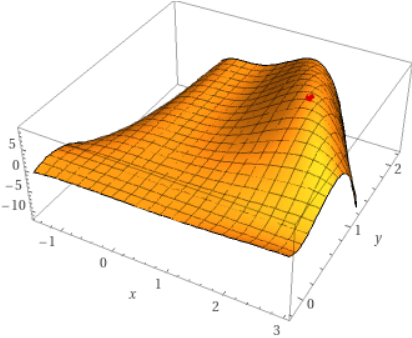
\includegraphics[width=0.5\linewidth]{pic/graph.png}}
\caption{График функции $z(x,y) = x^3y^2(4-x-y)$ с экстремумом в точке  $  \left(2, \frac{4}{3}\right)$.}
\center{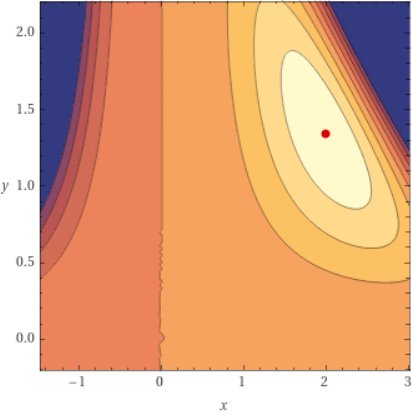
\includegraphics[width=0.5\linewidth]{pic/lines.png}}
\caption{Линии уровня $z(x,y) = x^3y^2(4-x-y)$ с экстремумом в точке  $  \left(2, \frac{4}{3}\right)$.}
\end{figure}


\newpage
\subsection{Численный метод}
Численный метод поиска экстремума реализован на основе \textit{градиентного спуска} со следующими заданными параметрами:\\
\\
1. Целевая точка (точка экстремума)  $  \left(2, \frac{4}{3}\right)$;\\
2. Точка старта (нулевое приближение)  $  \left(1, 1 \right)$;\\
3. Формула для вычисления следующего шага:
\begin{equation}
(x_{k+1}, y_{k+1})=(x_k, y_k) + a_k \,\,grad\,\, f(x_k, y_k)
\end{equation}
\textbf{Результат работы программы 1:}\\
1. Критерий останова: $\left| \Delta f \right| < \epsilon = 10^{-20}$\\
2. Число итериций: $1654$, $a_k = 0.001$\\
3. Время выполнения: $0.39569736$ c\\
4. Полученная точка: $(1.99999978, 1.33333354)$\\
5. Значение функции: $z = 9.48148148$\\
\begin{figure}[h]
\center{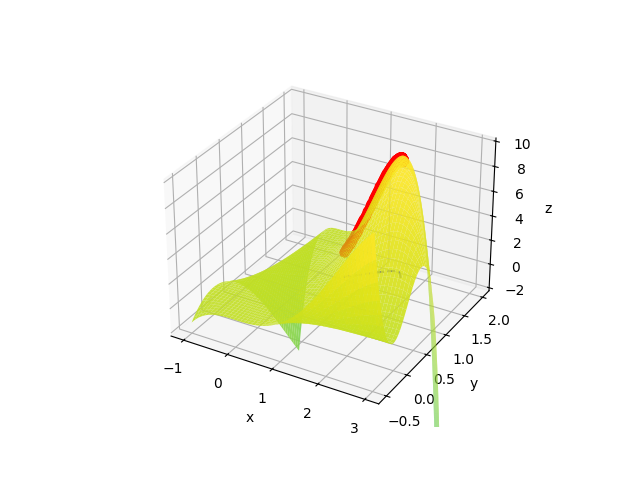
\includegraphics[width=0.9\linewidth]{pic/res_1.png}}
\caption{Результат работы программы 1.}
\end{figure}

\textbf{Результат работы программы 2:}\\
1. Критерий останова: $\| ( \Delta x_k, \Delta y_k  ) \| < \delta = 10^{-20}$\\
2. Число итериций: $3536$, $a_k = 0.001$\\
3. Время выполнения: $0.35638070$ c\\
4. Полученная точка: $(2., 1.33333333)$\\
5. Значение функции: $z = 9.48148148$\\
\begin{figure}[h]
\center{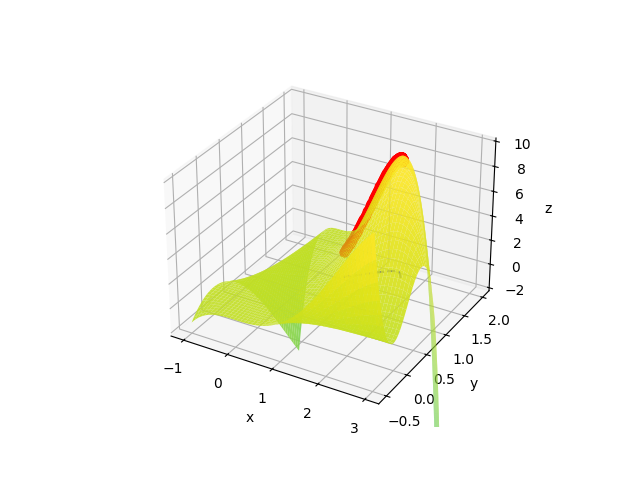
\includegraphics[width=0.9\linewidth]{pic/res_2.png}}
\caption{Результат работы программы 2.}
\end{figure}
\\
\textbf{Вывод:} по результатам выполнения программы с разными критериями останова можно сказать, что метод градиентного спуска дает одинаково хороший результат, как при условии малости приращения функции, так и при требовании малости приращения ее аргументов. Время выполнения отличается не сотые секунды, количество итериций во втором случае почти в 2 раза выше, но и результат поиска точки максимума точнее. Поэтому если говорить об эффективности, выбор критерия останова как $\| ( \Delta x_k, \Delta y_k  ) \| < \delta$, демонстрирует лучшие результаты.


\end{document}













